\documentclass[12pt]{article}
\usepackage{tikz}
\usepackage{xspace}
\usepackage{amsmath}
\usepackage{booktabs}
\usepackage{multicol}
\usepackage{graphicx}
\usetikzlibrary{arrows.meta}
\graphicspath{ {./images/} }
\pagestyle{empty}
\textwidth      165mm
\textheight     252mm
\topmargin      -18mm
\oddsidemargin  -2mm
\evensidemargin -2mm
\renewcommand{\baselinestretch}{0.97}
\renewcommand{\theenumi}{\alph{enumi}}
\newcommand{\impl}{\mathbin{\Rightarrow}}
\newcommand{\biim}{\mathbin{\Leftrightarrow}}
\newcommand\tab[1][1cm]{\hspace*{#1}}
\newcommand{\lto}{\mathbin{\to}}

\begin{document}

\begin{center}
{\sc The University of Melbourne
\\
School of Computing and Information Systems
\\ 
COMP30026 Models of Computation}
\bigskip \\
{\Large\bf Assignment 2, 2018}
\bigskip \\
Samuel Xu \\
Student No. 835273
\end{center}

\subsection*{Challenge 5 Answer}

Let $DFA (Q, \Sigma, \delta, q_0, F)$ and $PDA (Q', \Sigma', \Gamma, \delta', q_0', F')$ \\\\
The goal is to translate our $DFA$ to a 3-state $PDA$. This can be accomplished by creating a PDA similar to that of a naive search or graph traversal. \\
This process is possible as there are only two cases to account for:
\begin{enumerate}  
\item The current state is \textit{not} an accept state
\item The current state is an accept state
\end{enumerate} 
This results in a translation from any $DFA$ to a 3-state $PDA$; 
the first state of the $PDA$ being the \textit{initialisation state} ($q_I$), 
followed by the \textit{searching state} ($q_R$) and the \textit{accept state} ($q_A$).\\\\
First we start by defining our variables:\\\\
\textbf{DFA:} \\
Let $Q$ be a set of DFA states. \\
Let $\Sigma$ be a valid alphabet for our DFA. \\
Let $\delta$ be a valid set of transition functions for moving between states with a given input. \\
Let $q_0$ be the initial state of our DFA. \\
Let $F$ be a set of valid accept states for our DFA. \\\\
\textbf{PDA:} \\ 
Let $Q' = \{q_I, q_R, q_A\}$ \\
Let $\Sigma' = \Sigma_\epsilon$ \\
Let $\Gamma$ be a stack alphabet where $\Gamma = Q$ \\
Let $\delta'$ be the three transition functions between $q_I$, $q_R$, and $q_A$ \\ (following the form described in lecture 18 $\delta : Q \times \Sigma_\epsilon \times \Gamma_\epsilon \rightarrow \mathcal{P}(Q \times \Gamma_\epsilon)$;

$\delta : \{(q_I, \epsilon, \epsilon, \rightarrow q_R, q_0), (q_R, a, b, \rightarrow q_R, \delta(b, a)), (q_R, \epsilon, f \rightarrow q_A, \epsilon) \}$ \\
Let $q_0'$ be the starting state $\{q_I\}$ \\
Let $F'$ be the accept state $\{q_A\}$ \\
Let $a$ be a string input where $a \in \Sigma$ \\
Let $b$ be a state where $b \in Q$ \\
Let $f$ be an accept state where $f \in F$ \\\\

Now we may draw a PDA:\\

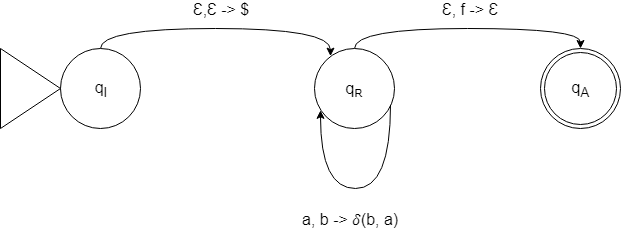
\includegraphics[width=\textwidth]{q5}

\end{document}